\documentclass{article}

% Language Setting
\usepackage[english]{babel}

% Set page size and margins
\usepackage[letterpaper,top=2cm,bottom=2cm,left=3cm,right=3cm,marginparwidth=1.75cm]{geometry}

% Useful Packages
\usepackage{amsmath}
\usepackage{graphicx}
\usepackage{listings}
\usepackage[colorlinks=true, allcolors=blue]{hyperref}

\title{Question 30: Power Station Problem}
\author{Alec Him}
\date{}

\begin{document}
\maketitle


\section{Introduction}
This document contains the mathematical derivation and calculations for solving the power station problem. The goal is to minimize the cost of the power line leading from the factory to the power station. 
\begin{figure}[h!]
    \centering
    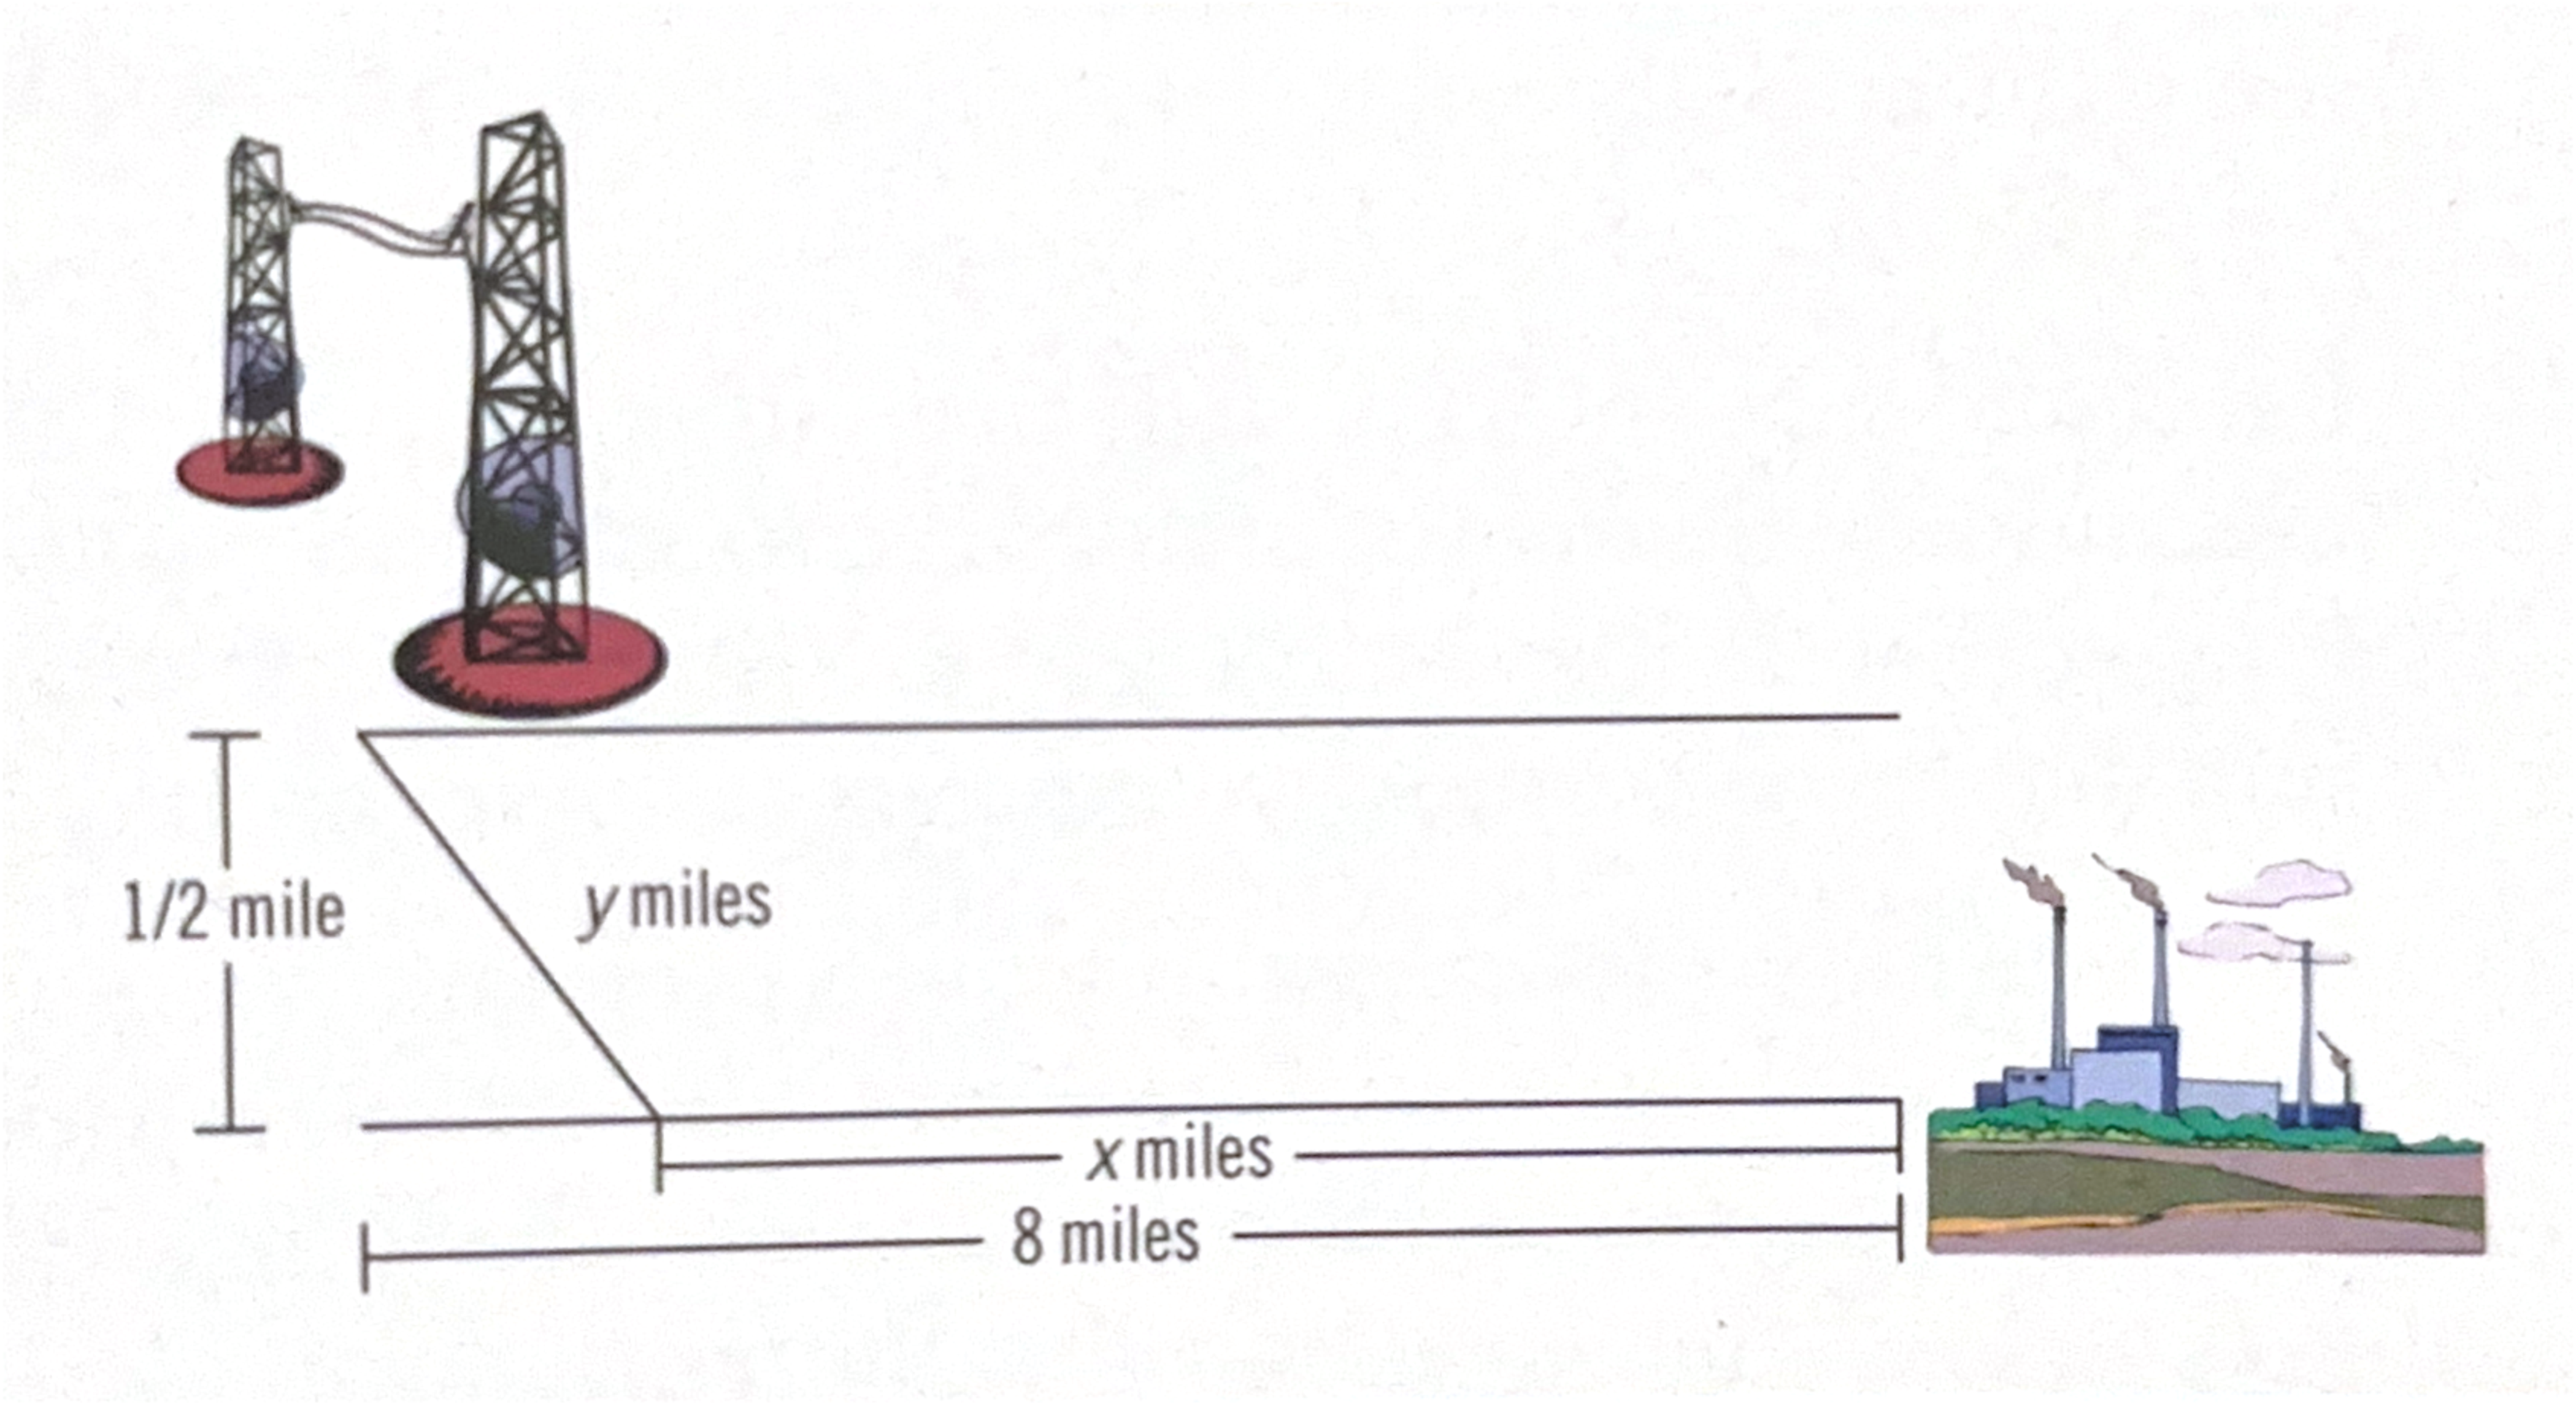
\includegraphics[width=0.6\textwidth]{Figure1.pdf}
    \caption{The factory is \( d \) mile(s), presented as 8 miles, downstream on the other side of the river from the power station, with the river being \( r \) mile(s), presented as 1/2 mile, wide.}
    \label{fig.Graph}
\end{figure}


\section{Variables}
\begin{itemize}
    \item \( d \): The distance downstream on the other side of the river (user inputted as \texttt{distance}).
    \item \( w \): The width of the river (user inputted as \texttt{width}).
    \item \( x \): The length of the power line on land.
    \item \( y \): The length of the power line under water.
    \item \( L \): The cost of the power line on land (user inputted as \texttt{landCost}).
    \item \( U \): The cost of the power line under water (user inputted as \texttt{waterCost}).
\end{itemize}


\section{Formulation and Derivation}
The total cost, \( C \), of the power lines is expressed by:
\begin{equation}
    C = (L \cdot x) + (U \cdot y)
\end{equation}
where:
\begin{equation}
    x = d - \left(\sqrt{y^2 - w^2}\right),\quad y = \sqrt{\left(d - x\right)^2 + w^2} 
\end{equation}
Expanding \( C \) with respect to \( x \):
\begin{align}
    C(x) &= (L \cdot x) + (U \cdot \left(\sqrt{\left(d - x\right)^2 + w^2}\right)) \\
\end{align}


\section{Minimization using Calculus}
To minimize \( C \), differentiate \( C \) with respect to \( x \) and set \( \frac{dC}{dx} \) = 0.
\begin{align*}
    \frac{dC}{dx} = C(x)' &= \frac{d}{dx}\left[(L \cdot x) + (U \cdot \left(\sqrt{\left(d - x\right)^2 + w^2}\right))\right] = 0 \\
    &= \frac{d}{dx}\left[L \cdot x\right] + \frac{d}{dx}\left[U \cdot \left(\sqrt{\left(d - x\right)^2 + w^2}\right)\right] = 0 \\
    &= L \cdot \frac{d}{dx}(x) + U \cdot \frac{d}{dx}\left(\sqrt{(d - x)^2 + w^2}\right) = 0 \\
    &= L + U \cdot \frac{1}{2}\left((d - x)^2 + w^2\right)^{\frac{1}{2} - 1} \cdot \frac{d}{dx}\left[(d - x)^2 + w^2\right] = 0 \\
    &= L + U \cdot \frac{1}{2 \cdot \sqrt{(d - x)^2 + w^2}} \cdot \frac{d}{dx}\left[(d - x)^2\right] + \frac{d}{dx}\left[w^2\right] = 0 \\
    &= L + U \cdot \frac{2 \cdot \left(d - x\right) \cdot \frac{d}{dx}\left[d - x\right] + 0}{2 \cdot \sqrt{(d - x)^2 + w^2}} = 0 \\
    &= L + U \cdot \frac{(d - x) \cdot \frac{d}{dx}\left[d\right] - \frac{d}{dx}\left[x\right]}{\sqrt{(d - x)^2 + w^2}} = 0 \\
    &= L + U \cdot -\frac{d - x}{\sqrt{(d - x)^2 + w^2}} = 0
\end{align*}
Solving for \( x \):
\begin{align*}
    -L = U \cdot -\frac{d - x}{\sqrt{(d - x)^2 + w^2}} \\
    \frac{L}{U} = \frac{d - x}{\sqrt{(d - x)^2 + w^2}} \\
    \frac{L}{U} \left(\sqrt{(d - x)^2 + w^2}\right) = d - x \\
    \left(\frac{L}{U}\right)^2 \left((d - x)^2 + w^2\right) = (d - x)^2 \\
    \frac{L^2}{U^2} (d - x)^2 + \frac{L^2}{U^2} w^2 = (d - x)^2 \\
    (d - x)^2 - \frac{L^2}{U^2} (d - x)^2 = \frac{L^2}{U^2} w^2 \\
    (d - x)^2 \left(1 - \frac{L^2}{U^2}\right) = \frac{L^2}{U^2} w^2 \\
    (d - x)^2 = \frac{L^2 \cdot w^2}{U^2 \left(1 - \frac{L^2}{U^2}\right)} \\
    (d - x)^2 = \frac{L^2 \cdot w^2}{U^2 - L^2} \\
    d - x = \frac{L \cdot w}{\sqrt{U^2 - L^2}} \\
    x = d - \frac{L \cdot w}{\sqrt{U^2 - L^2}}
\end{align*}


\section{Conclusion}
The derived formula for \( x \),
\begin{displaymath}
    x = d - \frac{L \cdot w}{\sqrt{U^2 - L^2}}
\end{displaymath}
determines the optimal land distance before transitioning to an underwater power line. By substituting \( x \) into
\begin{displaymath}
    y = \sqrt{(d - x)^2 + w^2}
\end{displaymath}
we obtain the corresponding underwater cable length, ensuring that the total cost
\begin{displaymath}
    C = Lx + Uy
\end{displaymath}
is minimized.

\end{document}